\subsection{Fuerza Bruta}
Como primera opci\'on para resolver el problema se encuentra el algor\'itmo de Fuerza Bruta que, tal como el nombre
da a suponer, es una forma poco inteligente de buscar una soluci\'on ya que implica recorrer todo el \'arbol de 
soluciones:

\begin{codebox}
    \Procname{\proc{ResolverFuerzaBruta}(int V, int[] S, int i, int n) \textcolor{red}{O($2^n$)}}
    \li \If $i == -1$ \textcolor{red}{O($1$)}
        \Then
    \li        \If $V == 0$ : \textcolor{red}{O($1$)}
                \Then
    \li             \Return $0$ \textcolor{red}{O($1$)}
    \li         \Else: 
    \li                 \Return $n+1$\footnote{Si el algor\'itmo devulve un n\'umero mayor que $n$ significa que no existe soluci\'on} \textcolor{red}{O($1$)}
                \End
                \End

    \li \Return min(ResolverFuerzaBruta($V$,$S$,$i-1$,$n$), \\
   $\quad\quad\quad\quad\quad$ $1 +$ResolverFuerzaBruta($V-S[i]$,$S$,$i-1$,$n$)) \textcolor{red}{O($2^n$)}

    \end{codebox}


\begin{figure}[H] 
\centering
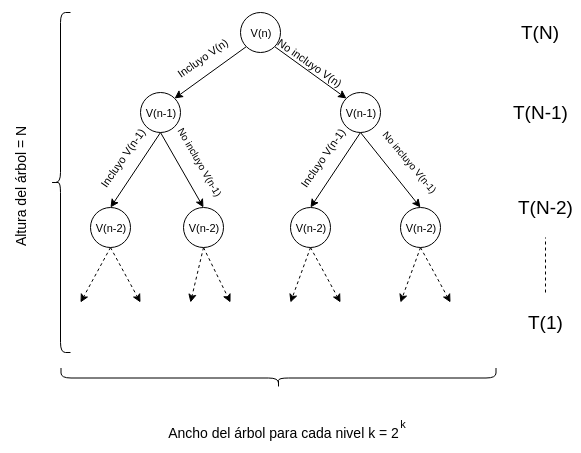
\includegraphics[width=.8\textwidth]{img/arbolRecurrencia.png}
\caption{\'Arbol de recurrencia}
\label{fig:arbolRecurrencia}
\end{figure}

Como la altura del \'arbol es de $n$ (el tama\~no del conjunto $S$) y el $\forall k, 1\leq k \leq n$ el ancho del
\'arbol para el nivel $k$ es de $2^k$, para recorrer todo el \'arbol se requieren:
\begin{equation}
    \sum_{i=0}^{n-1} 2^i*O(1) = \frac{2^{n}}{2-1} = 2^{n} \in O(2^n)
\end{equation}
Como se requieren $O(2^n)$ operaciones para investigar todas las soluciones y efectivamente se las investiga todas,
la complejidad del Fuerza Bruta es exactamente $O(2^n)$.

\subsection{Back Tracking}

\begin{codebox}
    \Procname{\proc{ResolverBackTracking}(int V, int[] S, int i, int n, int minParcial, int cardinalParcial) \textcolor{red}{O($2^n$)}} 
    % \li \If $i == -1$ \textcolor{red}{O($n*2^n$)}
    \li \If $cardinalParcial$ $>$ $minParcial$: \textcolor{red}{O($1$)}
        \Then
    \li        \Return $n+1$ \footnote{\label{bktrk}Si el algor\'itmo devulve un n\'umero mayor que $n$ significa que no existe soluci\'on} \End\textcolor{red}{O($1$)}
    \li \If $V == 0$: \textcolor{red}{O($1$)}
         \Then
    \li         $minParcial = cardinalParcial$ \textcolor{red}{O($1$)}
    \li         \Return $0$ \textcolor{red}{O($1$)}
    \End
    \li \If $i == -1$ \textcolor{red}{O($1$)}
        \Then
    \li                 \Return $n+1$ \textsuperscript{\ref{bktrk}} \textcolor{red}{O($1$)}
                \End
    \li \If $S[i]$ $>$ $V$: \textcolor{red}{O($1$)}
        \Then 
    \li         \Return  ResolverBackTracking($V$,$S$,$i-1$,$n$,$minParcial$,$cardinalParcial$)\textcolor{red}{O($2^n$)}
    \li    \Else:
    \li          \Return min(ResolverBackTracking($V$,$S$,$i-1$,$n$,$minParcial$,$cardinalParcial$),\textcolor{red}{O($2^n$)}
                            \\ $\qquad\qquad$$\qquad\quad\,\,$ $1+$ ResolverBackTracking($V-S[i]$,$S$,$i$,$n$,$minParcial$,$cardinalParcial+1$))



    \end{codebox}

\par Resulta f\'acil ver que la soluci\'on de Back Tracking es un caso especial del algor\'itmo de Fuerza Bruta,
salvo que gracias a las podas de \textit{optimalidad} y \textit{factibilidad} se evita investigar ciertas partes del
\'arbol de soluci\'on. A\'un as\'i, en el peor caso (por ejemplo un arreglo en el cual la suma de sus elementos no llega
a $V$) se termina comportando como Fuerza Bruta. Luego su complejidad resulta $O(2^n)$

\subsubsection{Poda por factibilidad}
\par La poda por \textit{factibilidad} se realiza en en la l\'inea 9 del pseudoc\'odigo. La misma consiste en
evaluar si el $S[i]$ es mayor estricto que el $V$. De as\'i serlo se excluye tal elemento en la soluci\'on ya que obviamente
har\'a que la suma de cualquier subconjunto que lo incluya exceder\'a el valor de $V$.


\subsubsection{Poda por optimalidad}
\par La poda por optimalidad se realiza en la l\'inea 1 del pseudoc\'odigo aunque las operaciones gracias a las
cuales funciona esta poda se realizan en las l\'ineas 4 y 12. En la primer l\'inea se evalua si el $cardinalParcial$
(el cardinal que lleva el subconjunto actual) es mayor estricto a $minParcial$ (el m\'inimo cardinal para el que
se encontr\'o un subconjunto cuya suma es exactamente $V$); de as\'i serlo, no tiene relevancia seguir evaluando
esa rama del \'arbol de soluciones ya que en caso de encontrar un subconjunto cuya suma sea $V$, su cardinal no ser\'a
el m\'inimo.
\par En la l\'inea 12, si se encontr\'o un subconjunto cuya suma sea $V$ (n\'otese que el $cardinalParcial$ debe
ser menor o igual al $minParcial$ gracias a la condici\'on en la l\'inea 1), $cardinalParcial$ pasa a ser el nuevo
$minParcial$ y se llega al caso base, por lo que se devuelve 0.
\par En la l\'inea 11 se busca el m\'inimo evaluan dos casos: incluir o no el elemento $S[i]$. N\'otese que en caso
de incluirlo el $cardinalParcial$ aumenta en 1.

\subsection{Programaci\'on Din\'amica}

\begin{codebox}
    \Procname{\proc{ResolverDinamica}(int V, int[] S, int i, int n, matriz resultados) \textcolor{red}{O($n*V$)}}
    \li \If $i == -1$  \textcolor{red}{O($1$)}
        \Then
    \li                 \Return $n+1$\footnote{\label{bktrk}Si el algor\'itmo devulve un n\'umero mayor que $n$ significa que no existe soluci\'on} \textcolor{red}{O($1$)}
                \End
    \li \If $noEstaDefinido(resultados[i][V]$):  \textcolor{red}{O($1$)}
        \Then 
    \li          \Return min(ResolverDinamica($V$,$S$,$i-1$,$n$,$resultados$,
                            \\ $\qquad\qquad$$\qquad\quad\,\,$ $1+$ResolverDinamica($V-S[i]$,$S$,$i-1$,$n$,$resultados$)) \textcolor{red}{O($n*V$)}
                            \End
    \li \Return resultados[i][vDeseado]  \textcolor{red}{O($1$)}
    \end{codebox}
% \par Para el caso de Programaci\'on Din\'amica, la complejidad resulta $O(n*V)$ ya que cada soluci\'on parcial 
% se calcula hasta una sola vez para luego almacerlo en una matriz de $n$ filas y $V$ columnas. Si la soluci\'on al
% problema de para un valor objetivo $V'$ y un una cantidad de elementos $i$, 
\par El algor\'itmo de Programaci\'on Din\'amica busca obtener una ventaja a partir de encarar al problema como
subproblemas recursivos pero, teniendo en cuenta que hay subproblemas que se calculan m\'as de una vez, se 
almacenan las subsoluciones  en una matriz de $n$ filas y $V$ columnas la cual es inicializada con ceros en
la primer columna (ya que acceder a esa columna implica que se lleg\'o a $V=0$, es decir, se encontr\'o un subconjunto v\'alido).
 El objetivo de guardar las soluciones es poder acceder a ellas
r\'apidamente. Es por esto que decidi\'i utilizar para almacenar las soluciones una matriz formada por un vector de 
vectores, permiti\'endome acceder en $O(1)$ a las soluciones ya calculadas.
\par Para un $V$ fijo, existen a lo sumo $n$ subproblemas para analizar. Luego, como $V$ o bien sigue igual o se le resta $S[i]$ ($S[i]\geq 0$ $\forall 1\leq i \leq n$)
existen a lo sumo $V$ valores objetivos que se investigan. Esto resulta en que se calculen $n*V$ soluciones, y dado que el resto de las operaciones de 
la funci\'on son constantes, la complejidad final resulta $O(n*V)$.
% \par La cantidad de posibles subproblemas es $n*V$: en cada llamada o bien se reduce $i$ (el indicador
% de cu\'al elemento de $S$ estoy analizando, $i<n$) o tambi\'en el valor $V$. Es por esto que para un $V$ existen a lo sumo $n$ subproblemas
% posibles.